\newpage
\section{Analysis}

In this section, the results of the case study are analysed to investigate the influence of different aspects on the optimal reliability indices, and the difference in result between the conventional and proposed approach.
First, the effect of different values for the shadow price is considered, and a connection is made between the two multi-objective approaches.
Next, the effect of varying the coefficients of variation in the probabilistic model of the structure and the additional damage costs $C_H$ on the optimal reliabilities is investigated, followed by a number of variants of the considered structure derived from \cite{Hingorani2023SustainabilityDesign}.
Finally, the ratio between the steel material cost and shadow-costed emissions is considered.
All these aspects are expected to influence the optimal reliability values indices, but the effect on the difference in results between the conventional and proposed augmented approaches is harder to predict.
This is represented by the difference between the conventional optimal reliability $\beta_{opt,C}$ and the augmented value $\beta_{opt,aug}$, here denoted as $\Delta \beta$:
\begin{equation}
    \label{eqn:delta_beta}
    \Delta \beta = \beta_{opt,C} - \beta_{opt,aug}
\end{equation}

\subsection{Shadow price $c_e$}

If the optimal reliability takes account of both cost and emissions, it is intuitively located between the optimal values of the separate objectives.
In the weighted sum approach, its location is governed by the shadow price: the larger $c_e$, the more $x_{opt,aug}$ moves from $x_{opt,C}$ towards $x_{opt,E}$, and the smaller $\beta_{opt,aug}$ becomes, so $\Delta \beta$ increases.

The effect of different shadow prices on the augmented optimal reliability is visualised in Figure \ref{fig:single_ce}, where the value of $\beta_{opt,aug}$ is plotted against the value of $c_e$.
The left panel shows the effect of a range of shadow prices generally found in literature, between 0 and 1 \EUR{} per kg CO\textsubscript{2}eq \citep{EuropeanInvestmentBank2025ShadowPricing, KamaliSaraji2024BridgingApplications, Wang2017TheIndustry,  WorldBank2025PriceDashboard}.
The right panel shows the theoretical effect of very large shadow prices, which would cause $\beta_{opt,aug}$ to approach $\beta_{opt,E}$, as the costs become negligible in $C_{aug}(x)$ compared to the emissions.
As noted, the shadow price can be interpreted in different ways.
Intuitively, it could be viewed as a literal price to be paid for emitted carbon, set through regulation or market mechanisms.
Alternatively, it could also be interpreted more abstractly, as a relative importance of emissions with respect to cost, independent of actual pricing.
If hypothetically, the emission reduction were considered more important than cost minimisation, an arbitrarily large value of $c_e$ could be used.
For consistency, in the remaining analyses a shadow price of 0.8 \EUR{}/kg CO\textsubscript{2}eq will be used as in the original case study.

For this and other more commonly found shadow prices, the effect on the optimal reliability index remains of similar order to the difference between target reliabilities between different combinations of cost and consequence classes given in ISO2394 \citep{iso2394}.
Thus, the reduction in $\beta_{opt}$ with respect to the monetary optimum, $\Delta \beta$, can be considered equal to a `partial class' for the range of shadow prices found in literature.
This could potentially be amplified by differential discounting \citep{Emmerling2019TheEmissions, Nestico2023AImpacts}, which would likely increase the additional `push' from the shadow-costed emissions with respect to the costs.

\begin{figure}[h!]
    \centering
    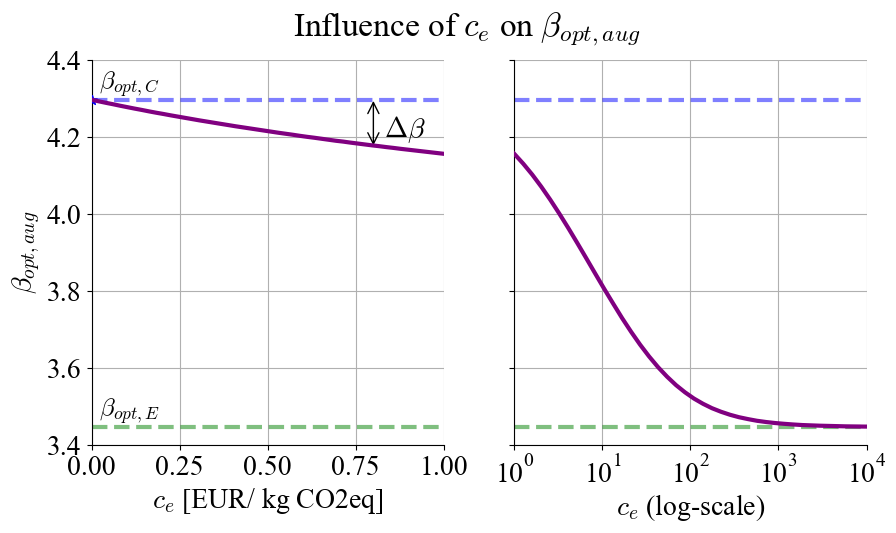
\includegraphics[width=0.7\textwidth]{Images/demo_ce.png}
    \caption{Augmented optimum dependent on shadow price. The left panel shows the effect for small but more realistic values of $c_e$, while the right panel shows how the optimal reliability approaches $\beta_{opt,E}$ for very large shadow prices.}
    \label{fig:single_ce}
\end{figure}

The weighted sum and $\varepsilon$-constraint approach can be connected through the Pareto front of Figure \ref{fig:pareto}.
Every point on this front is associated with a value for the shadow price $c_e$, a desired decrease in emissions $\Delta E_{desired}$ or allowed cost increase $\Delta C_{allowed}$ (which can be derived from the relative changes $\delta E_{desired}$ or $\delta C_{allowed}$).
This connection is visualised in Figure \ref{fig:triangle}: a constraint formulated with respect to the monetary optimum `cuts off' part of the Pareto front with either too much increase in costs or too little reduction in emissions.
The cut-off point in the remaining Pareto front then becomes the constrained optimum for the other objective.
Furthermore, the slope of the Pareto front at this point is then the reciprocal of the shadow costs, or equivalently, a line perpendicular to the Pareto front at this point has a slope equal to $c_e$.
This relation between the slope of a Pareto front and weight factors used in a weighted sum approach is a well-known phenomenon in multi-objective optimisation \cite{Deb2001Multi-objectiveAlgorithms}, and could be utilised to understand how the value of the shadow cost $c_e$, desired emission reduction $\delta E_{desired}$, or allowed cost increase $\delta C_{allowed}$ all interact with the value of the two objective functions and optimal reliability.


\begin{figure}[h!]
    \centering
    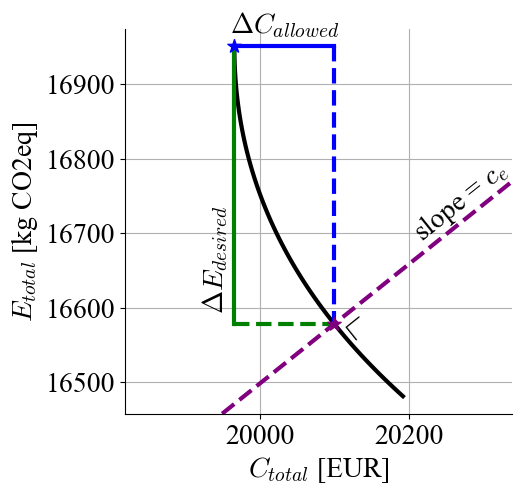
\includegraphics[width=0.55\textwidth]{Images/demo_triangle.png}
    \caption{Geometric interpretation of the shadow price, emission reduction and cost increase on the Pareto front}
    \label{fig:triangle}
\end{figure}


By considering that every point on the Pareto front of Figure \ref{fig:pareto} can be connected to a value of $\beta_{opt,aug}$.
Figure \ref{fig:single_3d} shows this connection: the reliability index $\beta$ corresponding to each value of $x$ in the region of interest is plotted as a curve hovering over the Pareto front associated with the same values of $x$.
For increasing $c_e$, $\delta E_{desired}$ or $\delta C_{allowed}$, the optimum moves along the Pareto front, starting at the blue star representing the costs-only optimum ($c_e = 0$), and moving towards the green star representing the emissions-only optimum ($c_e \rightarrow \infty$).
The costs at the optimum increase while the emissions decrease, and the optimal reliability $\beta_{opt,aug}$ `slides' downwards along the curve above the Pareto front.

\begin{figure}[h!]
    \centering
    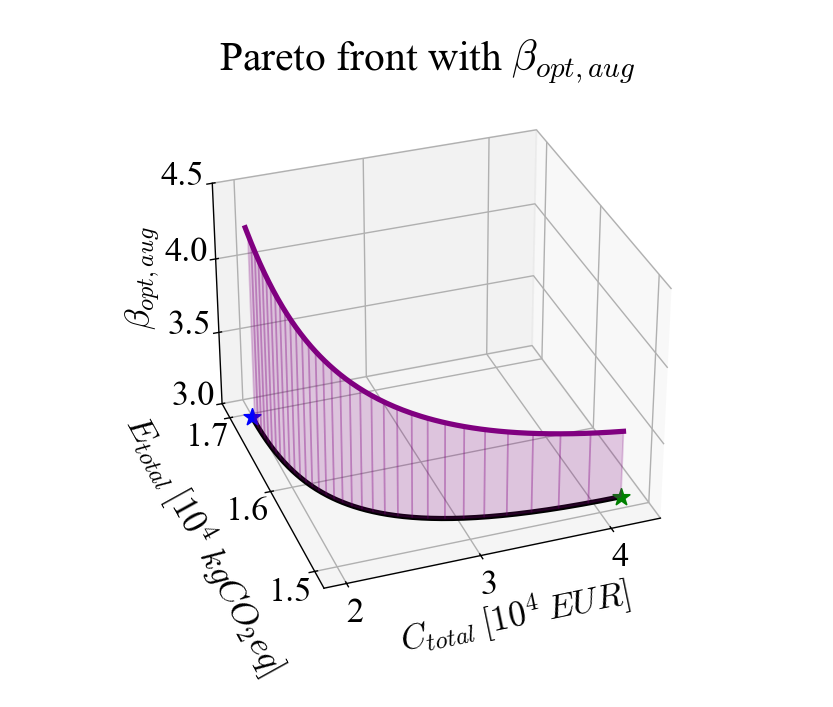
\includegraphics[width=0.7\textwidth]{Images/demo_3d.png}
    \caption{Visualisation of the interaction between the two objectives and the optimal reliability.}
    \label{fig:single_3d}
\end{figure}

For either of the optimisation approaches, some quantity needs to be chosen to find a single optimum from a two-objective problem, either a shadow price $c_e$ or a threshold value $C_{max}$ or $E_{max}$ setting a constraint.
The Pareto front connecting the two separate optima cannot, by itself, be used to find a single optimum.
However, its shape can be used to inform the choice of this quantity using the visualisations.
Which approach works best can depend on the local context and legislation, and in some cases, this may help choose the parameter value directly.
If a comprehensive `carbon tax' is active, this gives an intuitive choice for $c_e$.
If there is a general target for emission reduction, for the construction sector or for the economy in general, this could inform $\delta E_{desired}$, especially if the `status quo' based on monetary optimisation is used as a reference.
Finally, if some amount of money needs to be allocated for emission reductions, this can be used to set $\delta C_{allowed}$.

\clearpage
\subsection{Coefficients of variation}

An important aspect influencing the optimal reliability is the degree of uncertainty in the considered structure.
In general, the larger the variability of the loads and resistances, the larger $P_f$ is for a constant $x$.
This means a larger $x$ is needed to achieve the same reliability, so the cost of increasing safety effectively becomes larger (the `push' increases), leading to a smaller $\beta_{opt}$.
To investigate this effect in this case study, the three values of $\beta_{opt}$ for the considered beam are recalculated with differing coefficients of variations for three important variables in the limit state function: the yield strength $f_y$, permanent loads $g_{sw}$ and $g_{nsl}$, and live load $q_{live}$.
These are denoted as $V_f$, $V_g$ (for both permanent loads) and $V_q$, and were initially set to 0.05, 0.10 and 0.50 respectively \citep{Knibbe2026PlaceHolder, Hingorani2023SustainabilityDesign}.
Adjusting these values means the probabilistic model no longer follows the relevant background literature \citep{JCSS2000ProbabilisticDesign, Vrouwenvelder2024ReliabilityEurocodes}, so this should be considered as an academic exercise not representative of a real structure.
The adjusted coefficients of variation have therefore been chosen, somewhat arbitrarily,
The weighted sum approach is followed, keeping the shadow price $c_e$ at 0.8 \EUR{}/kg CO\textsubscript{2}eq.

Figure \ref{fig:cov} contains the result of this exercise.
As expected, larger coefficients of variation lead to smaller optimal reliabilities and vice versa.
% For the chosen values, the largest deviation from the values found using the original coefficients of variations is approximately 0.06 (the bottom line of Figure \ref{fig:cov}), half of the original difference found between $\beta_{opt,C}$ and $\beta_{opt,aug}$ using $c_e=0.8$.
Remarkably, $\Delta \beta$ is consistent across the different sets of coefficients of variation.
It appears that the reduction in optimal reliability with respect to the monetary optimum is unaffected by the degree of variability in the probabilistic model of the structure.
% As mentioned, this result can be linked to the constrained approach through the Pareto front.
% A similar analysis with a chosen value for $\delta E_{desired}$ or $\delta C_{allowed}$ would return identical results and is therefore not performed here.

\begin{figure}[h!]
    \centering
    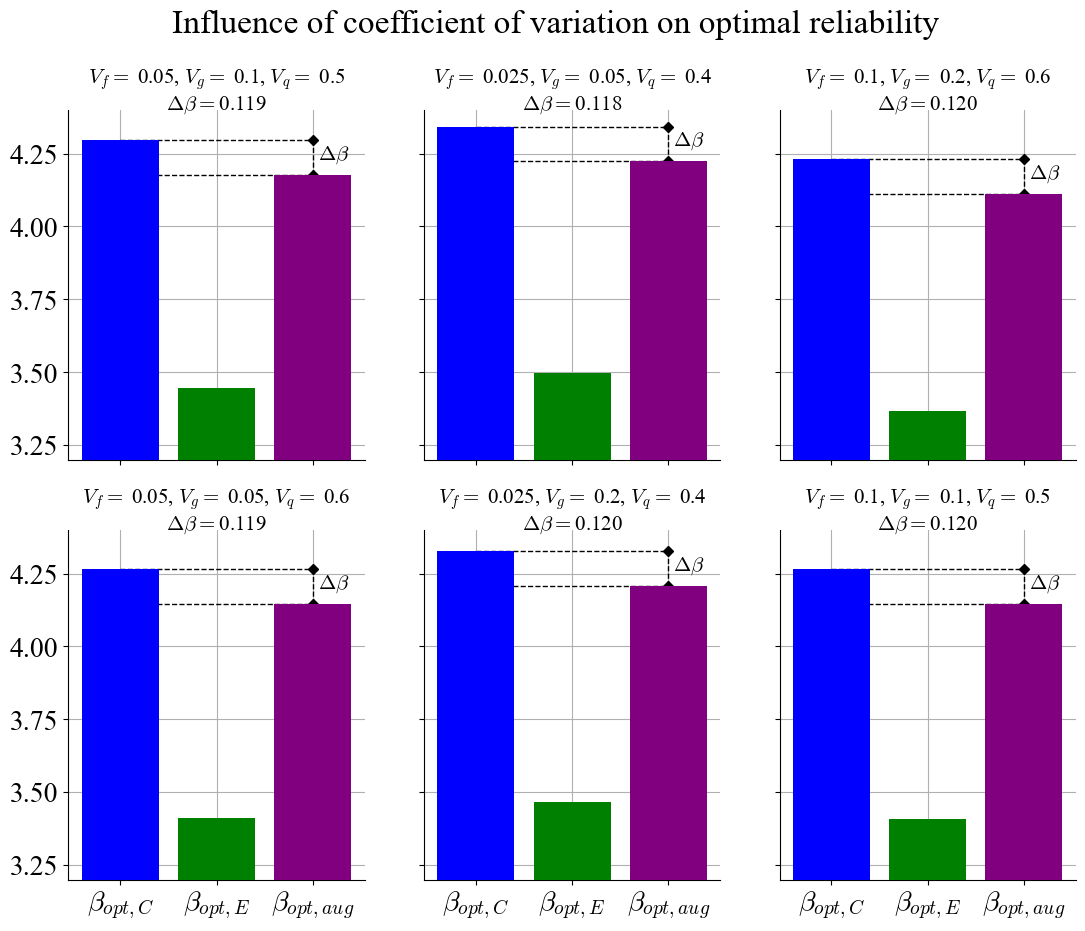
\includegraphics[width=0.85\textwidth]{Images/demo_cov_2.png}
    \caption{Influence of the coefficients of variation of the yield strength $V_f$, permanent load $V_g$, and live load $V_q$ pn the optimal reliability indices. A shadow price of 0.8 \EUR{}/kg CO\textsubscript{2}eq  has been used to find $\beta_{opt,aug}$}
    \label{fig:cov}
\end{figure}


\subsection{Damage costs $C_H$}

Next, the influence of the damage costs $C_H$ on the result is investigated.
As mentioned in Section \ref{sec:appraisal}, this value should include the term $SWTP \cdot N_f$ to represent human life risk, and a possible additional term $C_{H,other}$ to represent other indirect damage.
This latter term was originally neglected in the case study, as the material damage cost outside replacement of the beam is likely orders of magnitude smaller than the life risk costs for an office building.
However, it is worthwhile to investigate how hypothetical large values of $C_{H,other}$ would influence the optimal reliability, and especially the difference between the conventional and augmented optimum $\Delta \beta$.
For that reason, Figure \ref{fig:CH} presents $\beta_{opt,C}$ and $\beta_{opt,aug}$ varying across different orders of magnitude for the total $C_H$ ($\beta_{opt,E}$ is ignored here, as it is not influenced by $C_H$), including values smaller than $SWTP \cdot N_f$.
Again, this should be viewed as an academic exercise.

Both optimal reliability indices with increasing $C_H$, which is expected as the `pull' effect is strengthened.
Both appear to increase logarithmically with $C_H$, which is consistent with literature performing similar analyses \citep{Fischer2019OptimalDesign, Rackwitz2000OptimizationVerification}.
Notably, $\Delta \beta$ is constant once again.
It appears that the value of $C_H$, like the coefficients of variation, also does not influence the impact of the shadow costed emissions.


\begin{figure}[h!]
    \centering
    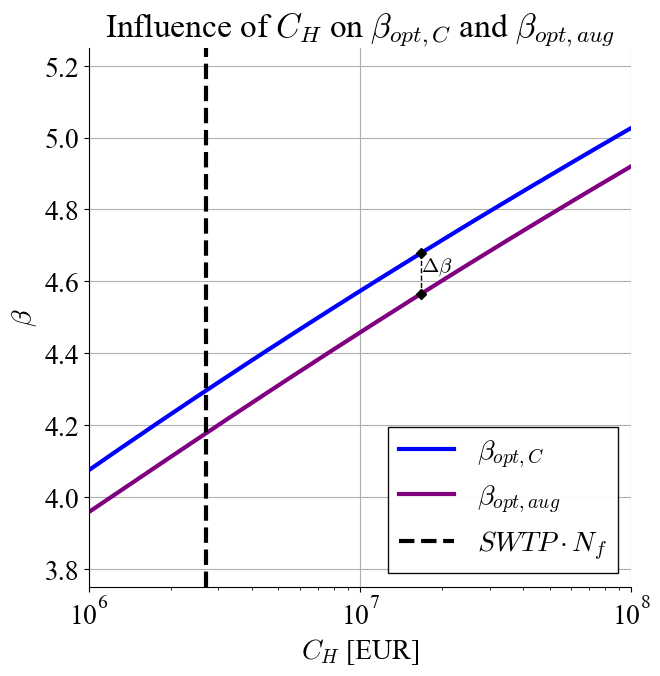
\includegraphics[width=0.65\textwidth]{Images/demo_C_H_sens.png}
    \caption{Optimal reliabilities dependent on the additional damage costs $C_H$. A shadow price of 0.8 \EUR{}/kg CO\textsubscript{2}eq has been used to find $\beta_{opt,aug}$}
    \label{fig:CH}
\end{figure}
\clearpage
\subsection{Variation of structure parameters}

The paper this case study has been adapted from \citep{Hingorani2023SustainabilityDesign} considered different variants of the considered structure by varying several parameters in the design problem: the beam length $L$, beam spacing $D$ underneath the floor slabs, the characteristic yield strength $f_{y,k}$, and two load ratios; $a_q$ setting the variable load $q_{live,k}$ to the total load $g_{sw,k} + g_{nsl,k} + q_{live,k}$, and $a_g$ setting the self-weight $g_{sw}$ to the permanent load $g_{sw,k} + g_{nsl,k}$ (all formulated in terms of characteristic values, which influence the mean values in the probabilistic model).
These variations resulted in a `population' of 50 different feasible designs (more details can be found in \cite{Hingorani2023SustainabilityDesign}).
To further investigate the generalisability of the case study results presented in the current work, the same optimisations have been performed on this population, resulting in 50 different values of $\beta_{opt,C}$, $\beta_{opt,E}$, $\beta_{opt,aug}$ (given $c_e=$0.80 \EUR{}/CO\textsubscript{2}eq), and the derived $\Delta \beta$.
Figure \ref{fig:population} and Table \ref{tab:population_stats} display the empirical cumulative distribution functions (CDF) and general statistics of these results.

All three optimal reliability indices are reasonably constant across the different variants, with the environmental optimum having somewhat more variance than the other two.
This is likely caused by the additional failure emissions $E_H$ which depend on both the floor are supported by the beam, set by the length $L$ and spacing $D$, as well as the load ratios $a_q$ and $a_g$.
The additional failure costs, $C_H$, depend only on the floor area and not the load ratios, hence this parameter varies to a lesser degree across the different variants in the population than $E_H$, and so does its `pull' effect on the respective optimal reliability.

The distribution of the augmented optimal reliability appears similar to that of the monetary optimum, shifted approximately 0.12 to the left.
This corresponds to the value of $\Delta \beta$ found in the original case study, which is also rather stable across this population of variants.
From this analysis, it appears that $\Delta \beta$ is reasonably consistent across different variants of the same structure, in terms of supported area, characteristic load ratios and material strength.


\begin{figure}[h!]
    \centering
    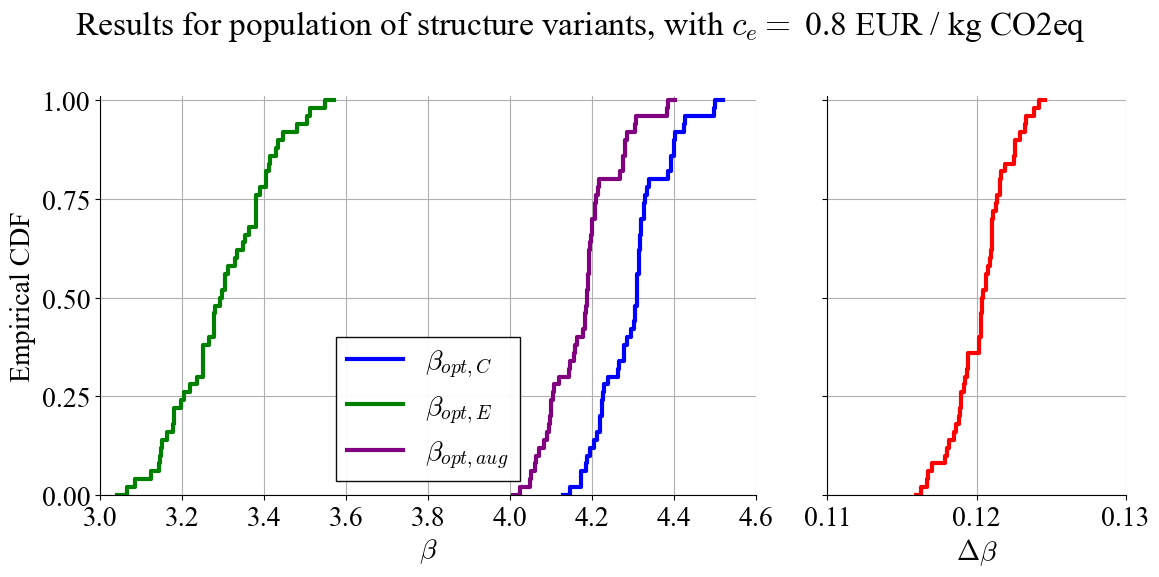
\includegraphics[width=0.85\textwidth]{Images/demo_population.png}
    \caption{Empirical cumulative distribution of optimal reliabilities (left) and $\Delta \beta$ (right) for a population of structure variants. A shadow price of 0.8 \EUR{}/kg CO\textsubscript{2}eq has been used to find $\beta_{opt,aug}$ and $\Delta \beta$}
    \label{fig:population}
\end{figure}

\begin{table}[]
    \centering
    \begin{tabular}{c|c|c|c|c}
         &  $\beta_{opt,C}$ & $\beta_{opt,E}$&$\beta_{opt,aug}$ &$\Delta \beta$\\ \hline
         Min& 
     4.15& 3.07&4.02 &0.116\\
 Median& 4.31& 3.30&4.19 &0.120\\
 Max& 4.50& 3.55&4.38 &0.124\\
 Mean& 4.30& 3.30&4.18 &0.120\\
 Std.dev.& 0.0815& 0.1161&0.083 &0.00185\\
 CoV& 0.019& 0.035&0.020 &0.015\\\end{tabular}
    \caption{Statistics of the optimal reliability indices of the population of structure variants}
    \label{tab:population_stats}
\end{table}

\subsection{Relation emission to material cost}

It has been shown that both the conventional and augmented optimal reliability indices are sensitive to the coefficients of variation, failure costs, and structural parameters.
However, $\Delta \beta$ is not affected as much, instead being determined by the shadow price $c_e$ as Figure \ref{fig:single_ce} shows.
An alternative view can be adopted by considering the shadow price and emissions of the structural material in relation to its monetary cost.
An \emph{emission-cost ratio} can then be defined as $c_e \cdot E_1 / C_1$ (unitless), and for the final analysis of this section, the effect of this ratio on $\Delta \beta$ is investigated.
A reasonable range for this ratio has been estimated based on various sources for the steel price \citep{bauforumstahle.V.2026BaukostenBauforumstahl, Bouwenmetstaal2024CostComponents, BritishConstructionalSteelworkAssociationCostSteelConstruction.info}, embodied emission of steel \citep{TATASteel2017BenefitsOwnership, WorldSteelAssociation2021ClimateSteel, OveArupPartners2023BuildingsSteel}, and carbon shadow price \citep{WorldBank2025PriceDashboard, EuropeanInvestmentBank2025ShadowPricing, Wang2017TheIndustry}.

Figure \ref{fig:ratio} shows the result.
A similar analysis has also been performed considering a reinforced concrete beam under the floor instead of a steel profile.
The parameters of this alternative case study are given in 

This is similar to the analysis behind Figure \ref{fig:single_ce}, where the shadow price $c_e$ was varied and the `pull'-term $c_e (E_{const}(x) + E_H) \frac{P_f(x)}{\gamma}$ in $E_{total}$ also changes.
Here, the focus is on the `push'-effect is varied in both objective functions, but the result is similar: $\Delta \beta$ increases approximately linearly with the emission-cost ratio.
The interpretation is different, however: while $c_e$ can (as mentioned) be considered a general weight factor representing the relative importance of the two objective functions in their entirety, the emission-cost ratio represents the environmental impact of the specific structural material relative to its monetary costs.
This is an important distinction, especially when considering the impact of the proposed approach across different structures.
If one structure is relatively cheap (low $C_1$) but emission-intensive (larger $E_1$) compared to another, it would have a larger emission-cost ratio and the proposed augmented optimisation would thus result in a larger $\Delta \beta$, even if the shadow price $c_e$ applied in both optimisations is the same.
It is then not the relative weight of emissions in general, but the difference in environmental impact relative to cost \emph{for the specific structure} that determines how the optimal reliability should change when emissions are considered.

\begin{figure}[h!]
    \centering
    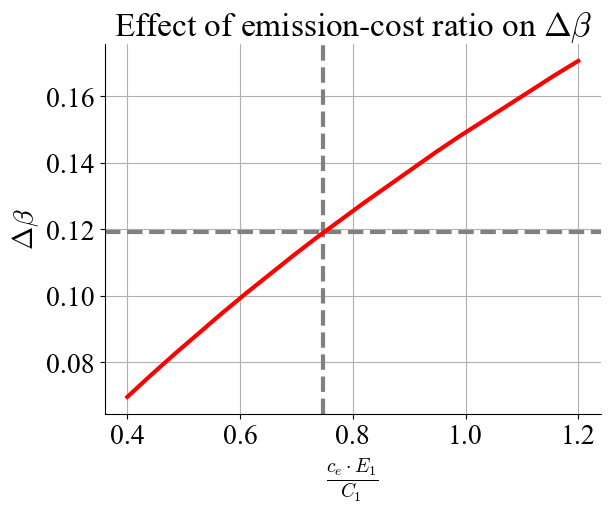
\includegraphics[width=0.65\textwidth]{Images/demo_ratio.png}
    \caption{$\Delta \beta$ as a function of the unitless ratio between shadow-costs and monetary costs of steel. The initial ratio and its outcome are marked.}
    \label{fig:ratio}
\end{figure}

Concrete version

emissions based on \citep{InformationsZentrumBetonGmbH2023BetonEPD-IZB-20230328-IBG1-DE}, 0.078 kgCO2 / kg C30 concrete
cost based on \citep{UniconPRICE2024}, 0,104 UER / kg C30 concrete